
\documentclass[]{article}
\usepackage[utf8]{inputenc}
\usepackage[usenames,dvipsnames]{xcolor}
\usepackage{fullpage}
\usepackage[upright]{fourier}
\usepackage{tkz-graph}
\usepackage{fancyhdr}
\usetikzlibrary{arrows}
\begin{document}

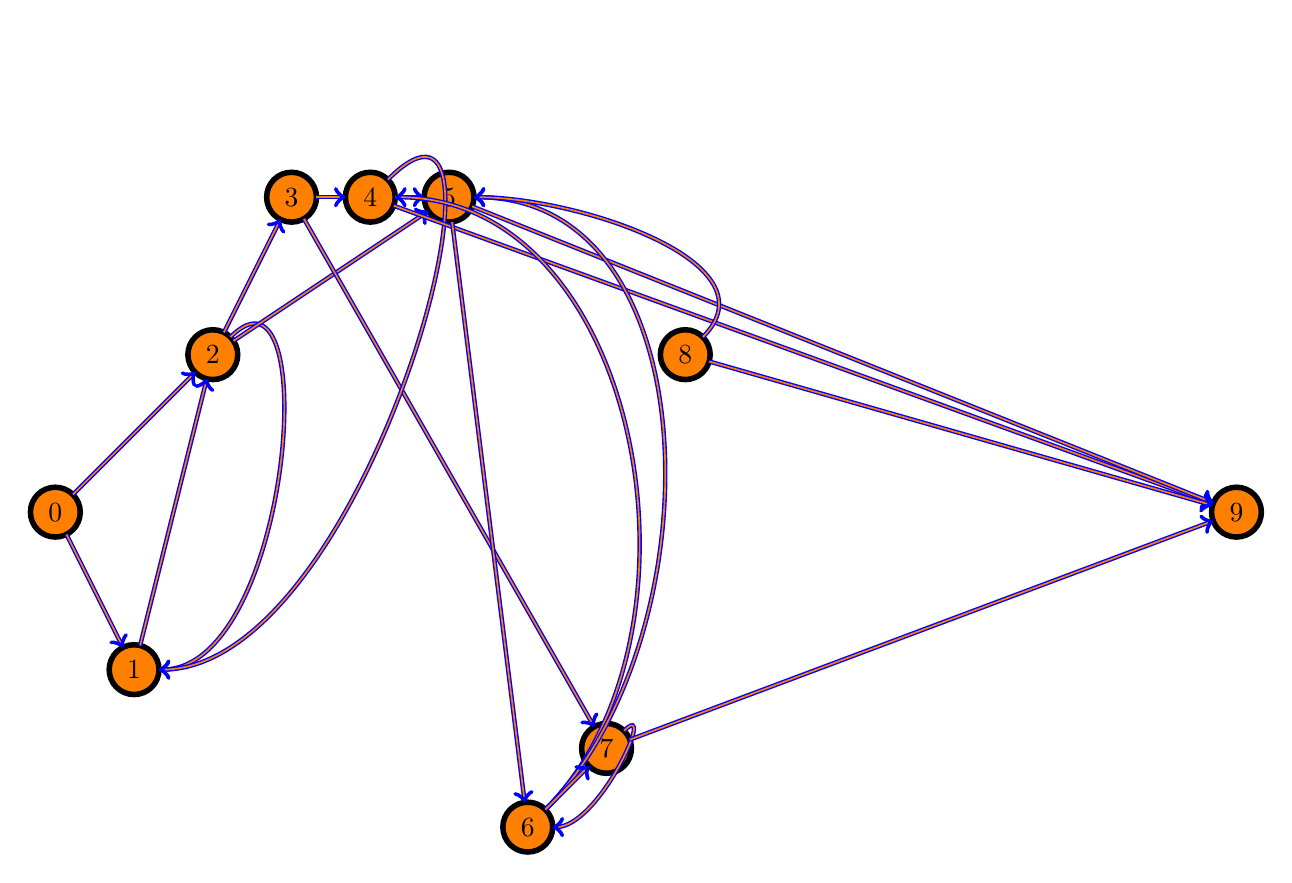
\begin{tikzpicture}
\SetVertexNormal[Shape      = circle,
FillColor  = orange,
LineWidth  = 2pt]
\SetUpEdge[lw         = 0.5pt,
color      = black,
labelcolor = white,
labeltext  = red,
labelstyle = {sloped,text=blue}]
\tikzstyle{TempStyle}=[double = orange]
\Vertex[x=-10, y=8]{0}
\Vertex[x=-9, y=6]{1}
\Vertex[x=-8, y=10]{2}
\Vertex[x=-7, y=12]{3}
\Vertex[x=-6, y=12]{4}
\Vertex[x=-5, y=12]{5}
\Vertex[x=-4, y=4]{6}
\Vertex[x=-3, y=5]{7}
\Vertex[x=-2, y=10]{8}
\Vertex[x=5, y=8]{9}
\tikzset{EdgeStyle/.style={->,TempStyle,relative=false,right=60,color=blue}}
\Edge(0)(1)
\tikzset{EdgeStyle/.style={->,TempStyle,relative=false,right=60,color=blue}}
\Edge(0)(2)
\tikzset{EdgeStyle/.style={->,TempStyle,relative=false,right=60,color=blue}}
\Edge(1)(2)
\tikzset{EdgeStyle/.style={->,TempStyle,relative=false,left=60,color=blue,in=0,draw}}
\Edge(2)(1)
\tikzset{EdgeStyle/.style={->,TempStyle,relative=false,right=60,color=blue}}
\Edge(2)(3)
\tikzset{EdgeStyle/.style={->,TempStyle,relative=false,right=60,color=blue}}
\Edge(2)(5)
\tikzset{EdgeStyle/.style={->,TempStyle,relative=false,right=60,color=blue}}
\Edge(3)(4)
\tikzset{EdgeStyle/.style={->,TempStyle,relative=false,right=60,color=blue}}
\Edge(3)(7)
\tikzset{EdgeStyle/.style={->,TempStyle,relative=false,left=60,color=blue,in=0,draw}}
\Edge(4)(1)
\tikzset{EdgeStyle/.style={->,TempStyle,relative=false,right=60,color=blue}}
\Edge(4)(5)
\tikzset{EdgeStyle/.style={->,TempStyle,relative=false,right=60,color=blue}}
\Edge(4)(9)
\tikzset{EdgeStyle/.style={->,TempStyle,relative=false,right=60,color=blue}}
\Edge(5)(6)
\tikzset{EdgeStyle/.style={->,TempStyle,relative=false,right=60,color=blue}}
\Edge(5)(9)
\tikzset{EdgeStyle/.style={->,TempStyle,relative=false,left=60,color=blue,in=0,draw}}
\Edge(6)(4)
\tikzset{EdgeStyle/.style={->,TempStyle,relative=false,left=60,color=blue,in=0,draw}}
\Edge(6)(5)
\tikzset{EdgeStyle/.style={->,TempStyle,relative=false,right=60,color=blue}}
\Edge(6)(7)
\tikzset{EdgeStyle/.style={->,TempStyle,relative=false,left=60,color=blue,in=0,draw}}
\Edge(7)(6)
\tikzset{EdgeStyle/.style={->,TempStyle,relative=false,right=60,color=blue}}
\Edge(7)(9)
\tikzset{EdgeStyle/.style={->,TempStyle,relative=false,left=60,color=blue,in=0,draw}}
\Edge(8)(5)
\tikzset{EdgeStyle/.style={->,TempStyle,relative=false,right=60,color=blue}}
\Edge(8)(9)
\end{tikzpicture}\\
\begin{center}\begin{tabular}{l c}\\
\textcolor{orange}{\LARGE$\rightarrow$} & Chemin \\
 \textcolor{red}{\LARGE$\rightarrow$} & Créations arcs\\
 \textcolor{green}{\LARGE$\rightarrow$} & Modification flot\\
\end{tabular}
\end{center}
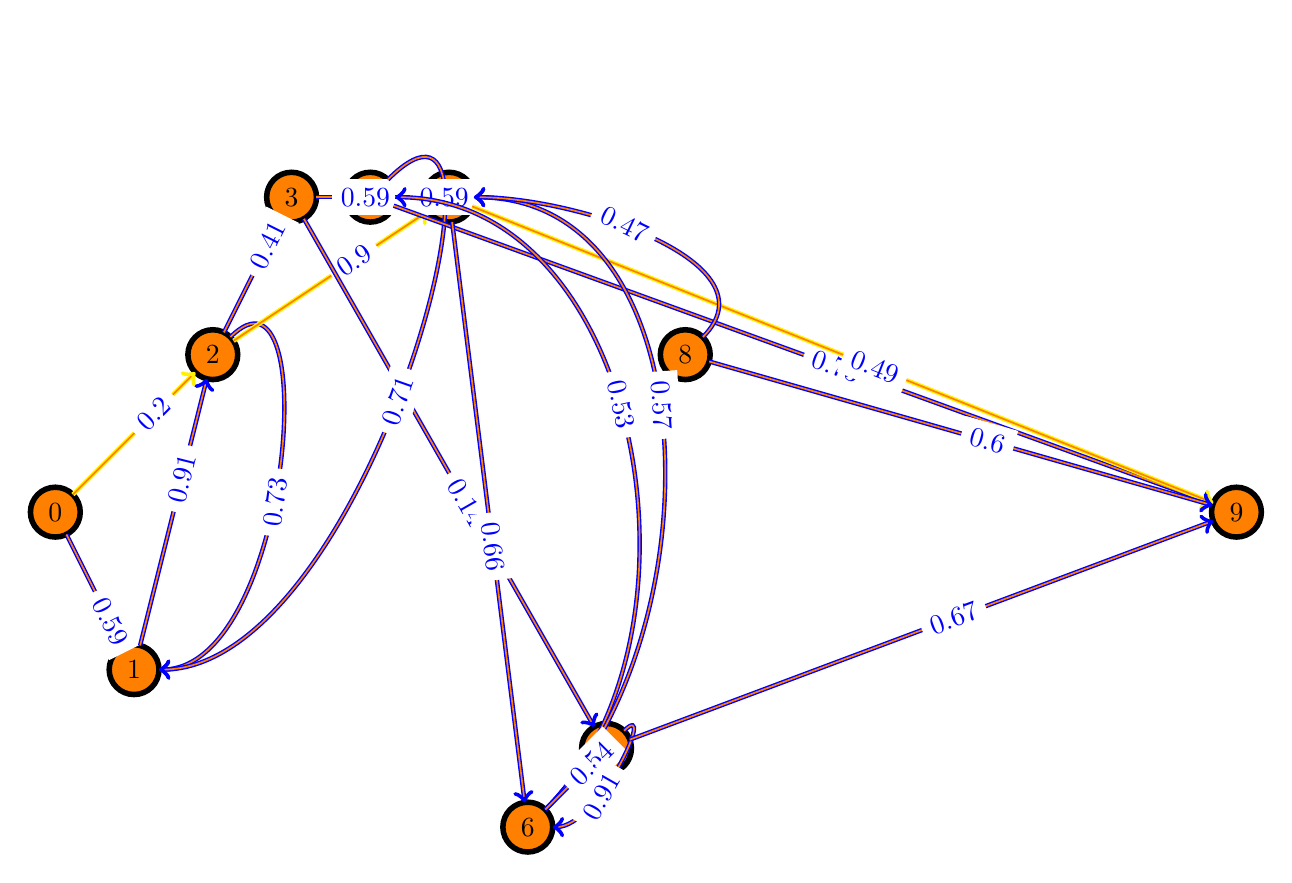
\begin{tikzpicture}
\SetVertexNormal[Shape      = circle,
FillColor  = orange,
LineWidth  = 2pt]
\SetUpEdge[lw         = 0.5pt,
color      = black,
labelcolor = white,
labeltext  = red,
labelstyle = {sloped,text=blue}]
\tikzstyle{TempStyle}=[double = orange]
\Vertex[x=-10, y=8]{0}
\Vertex[x=-9, y=6]{1}
\Vertex[x=-8, y=10]{2}
\Vertex[x=-7, y=12]{3}
\Vertex[x=-6, y=12]{4}
\Vertex[x=-5, y=12]{5}
\Vertex[x=-4, y=4]{6}
\Vertex[x=-3, y=5]{7}
\Vertex[x=-2, y=10]{8}
\Vertex[x=5, y=8]{9}
\tikzset{EdgeStyle/.style={->,TempStyle,relative=false,right=60,color=blue}}
\Edge[label=$0.59$](0)(1)
\tikzset{EdgeStyle/.style={->,TempStyle,relative=false,right=60,color=yellow}}
\Edge[label=$0.2$](0)(2)
\tikzset{EdgeStyle/.style={->,TempStyle,relative=false,right=60,color=blue}}
\Edge[label=$0.91$](1)(2)
\tikzset{EdgeStyle/.style={->,TempStyle,relative=false,left=60,color=blue,in=0,draw}}
\Edge[label=$0.73$](2)(1)
\tikzset{EdgeStyle/.style={->,TempStyle,relative=false,right=60,color=blue}}
\Edge[label=$0.41$](2)(3)
\tikzset{EdgeStyle/.style={->,TempStyle,relative=false,right=60,color=yellow}}
\Edge[label=$0.9$](2)(5)
\tikzset{EdgeStyle/.style={->,TempStyle,relative=false,right=60,color=blue}}
\Edge[label=$0.59$](3)(4)
\tikzset{EdgeStyle/.style={->,TempStyle,relative=false,right=60,color=blue}}
\Edge[label=$0.14$](3)(7)
\tikzset{EdgeStyle/.style={->,TempStyle,relative=false,left=60,color=blue,in=0,draw}}
\Edge[label=$0.71$](4)(1)
\tikzset{EdgeStyle/.style={->,TempStyle,relative=false,right=60,color=blue}}
\Edge[label=$0.59$](4)(5)
\tikzset{EdgeStyle/.style={->,TempStyle,relative=false,right=60,color=blue}}
\Edge[label=$0.73$](4)(9)
\tikzset{EdgeStyle/.style={->,TempStyle,relative=false,right=60,color=blue}}
\Edge[label=$0.66$](5)(6)
\tikzset{EdgeStyle/.style={->,TempStyle,relative=false,right=60,color=yellow}}
\Edge[label=$0.49$](5)(9)
\tikzset{EdgeStyle/.style={->,TempStyle,relative=false,left=60,color=blue,in=0,draw}}
\Edge[label=$0.53$](6)(4)
\tikzset{EdgeStyle/.style={->,TempStyle,relative=false,left=60,color=blue,in=0,draw}}
\Edge[label=$0.57$](6)(5)
\tikzset{EdgeStyle/.style={->,TempStyle,relative=false,right=60,color=blue}}
\Edge[label=$0.54$](6)(7)
\tikzset{EdgeStyle/.style={->,TempStyle,relative=false,left=60,color=blue,in=0,draw}}
\Edge[label=$0.91$](7)(6)
\tikzset{EdgeStyle/.style={->,TempStyle,relative=false,right=60,color=blue}}
\Edge[label=$0.67$](7)(9)
\tikzset{EdgeStyle/.style={->,TempStyle,relative=false,left=60,color=blue,in=0,draw}}
\Edge[label=$0.47$](8)(5)
\tikzset{EdgeStyle/.style={->,TempStyle,relative=false,right=60,color=blue}}
\Edge[label=$0.6$](8)(9)
\end{tikzpicture}\\
\begin{center}\begin{tabular}{l c}\\
\textcolor{orange}{\LARGE$\rightarrow$} & Chemin \\
 \textcolor{red}{\LARGE$\rightarrow$} & Créations arcs\\
 \textcolor{green}{\LARGE$\rightarrow$} & Modification flot\\
\end{tabular}
\end{center}
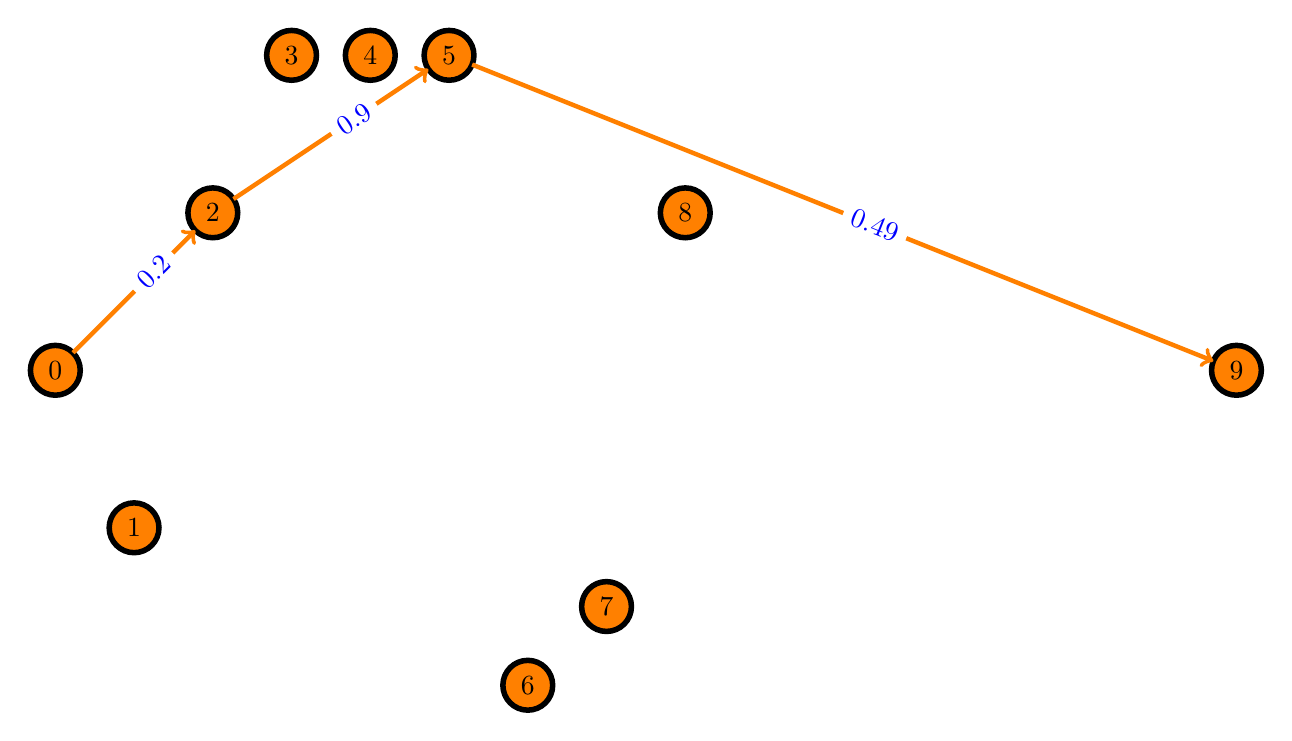
\begin{tikzpicture}
\SetVertexNormal[Shape      = circle,
FillColor  = orange,
LineWidth  = 2pt]
\SetUpEdge[lw         = 0.5pt,
color      = black,
labelcolor = white,
labeltext  = red,
labelstyle = {sloped,text=blue}]
\tikzstyle{TempStyle}=[double = orange]
\Vertex[x=-10, y=8]{0}
\Vertex[x=-9, y=6]{1}
\Vertex[x=-8, y=10]{2}
\Vertex[x=-7, y=12]{3}
\Vertex[x=-6, y=12]{4}
\Vertex[x=-5, y=12]{5}
\Vertex[x=-4, y=4]{6}
\Vertex[x=-3, y=5]{7}
\Vertex[x=-2, y=10]{8}
\Vertex[x=5, y=8]{9}
\tikzset{EdgeStyle/.style={->,TempStyle,relative=false,right=60,color=orange}}
\Edge[label=$0.2$](0)(2)
\tikzset{EdgeStyle/.style={->,TempStyle,relative=false,right=60,color=orange}}
\Edge[label=$0.9$](2)(5)
\tikzset{EdgeStyle/.style={->,TempStyle,relative=false,right=60,color=orange}}
\Edge[label=$0.49$](5)(9)
\end{tikzpicture}\\
\begin{center}\begin{tabular}{l c}\\
\textcolor{orange}{\LARGE$\rightarrow$} & Chemin \\
 \textcolor{red}{\LARGE$\rightarrow$} & Créations arcs\\
 \textcolor{green}{\LARGE$\rightarrow$} & Modification flot\\
\end{tabular}
\end{center}
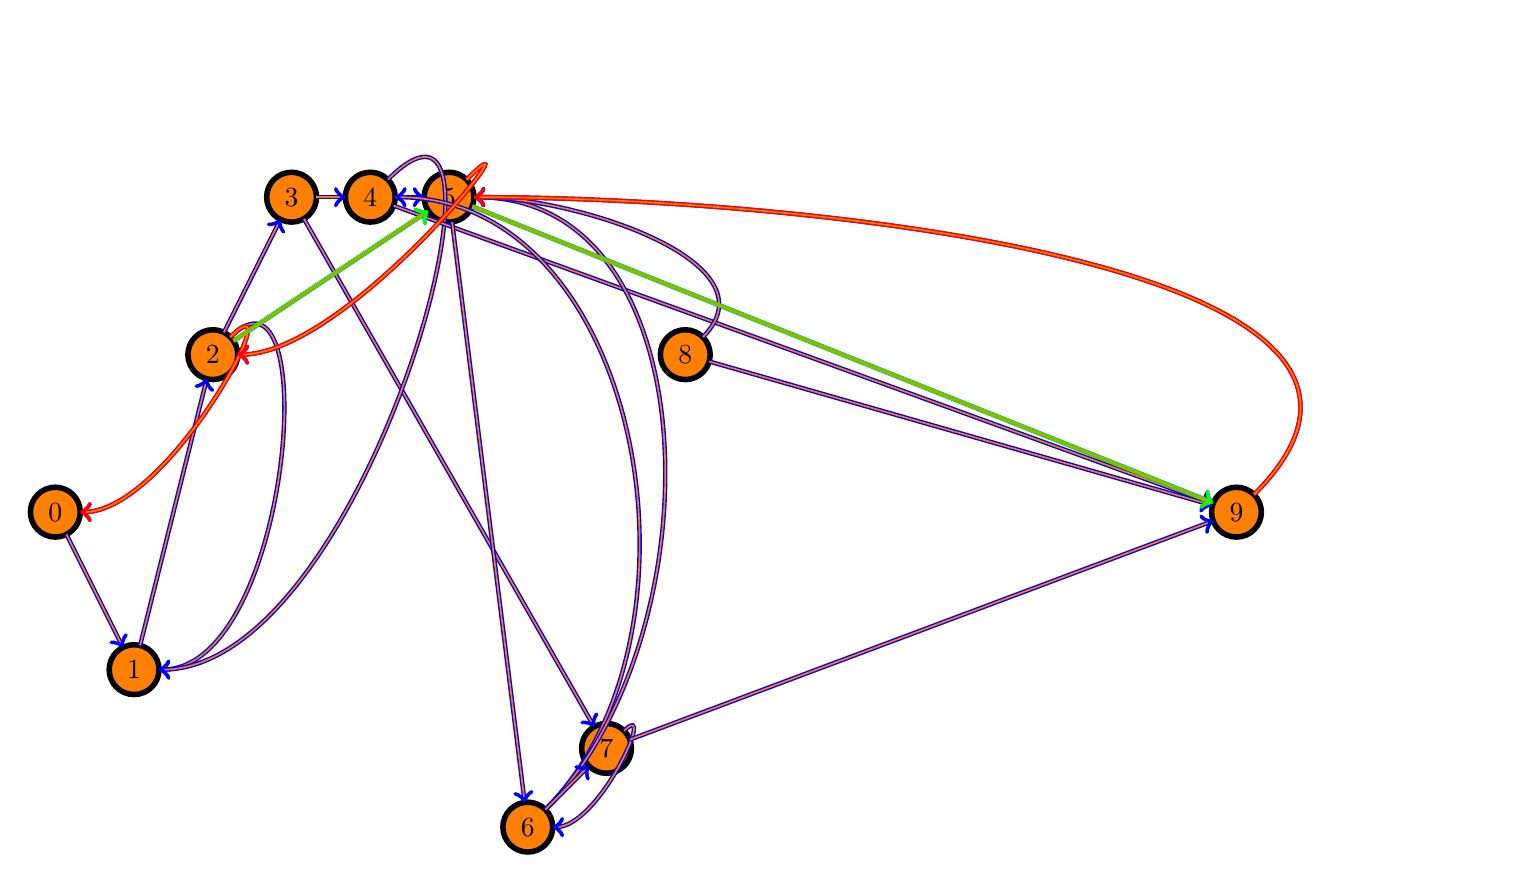
\begin{tikzpicture}
\SetVertexNormal[Shape      = circle,
FillColor  = orange,
LineWidth  = 2pt]
\SetUpEdge[lw         = 0.5pt,
color      = black,
labelcolor = white,
labeltext  = red,
labelstyle = {sloped,text=blue}]
\tikzstyle{TempStyle}=[double = orange]
\Vertex[x=-10, y=8]{0}
\Vertex[x=-9, y=6]{1}
\Vertex[x=-8, y=10]{2}
\Vertex[x=-7, y=12]{3}
\Vertex[x=-6, y=12]{4}
\Vertex[x=-5, y=12]{5}
\Vertex[x=-4, y=4]{6}
\Vertex[x=-3, y=5]{7}
\Vertex[x=-2, y=10]{8}
\Vertex[x=5, y=8]{9}
\tikzset{EdgeStyle/.style={->,TempStyle,relative=false,right=60,color=blue}}
\Edge(0)(1)
\tikzset{EdgeStyle/.style={->,TempStyle,relative=false,right=60,color=blue}}
\Edge(1)(2)
\tikzset{EdgeStyle/.style={->,TempStyle,relative=false,left=60,color=blue,in=0,draw}}
\Edge(2)(0)
\tikzset{EdgeStyle/.style={->,TempStyle,relative=false,left=60,color=blue,in=0,draw}}
\Edge(2)(1)
\tikzset{EdgeStyle/.style={->,TempStyle,relative=false,right=60,color=blue}}
\Edge(2)(3)
\tikzset{EdgeStyle/.style={->,TempStyle,relative=false,right=60,color=blue}}
\Edge(2)(5)
\tikzset{EdgeStyle/.style={->,TempStyle,relative=false,right=60,color=blue}}
\Edge(3)(4)
\tikzset{EdgeStyle/.style={->,TempStyle,relative=false,right=60,color=blue}}
\Edge(3)(7)
\tikzset{EdgeStyle/.style={->,TempStyle,relative=false,left=60,color=blue,in=0,draw}}
\Edge(4)(1)
\tikzset{EdgeStyle/.style={->,TempStyle,relative=false,right=60,color=blue}}
\Edge(4)(5)
\tikzset{EdgeStyle/.style={->,TempStyle,relative=false,right=60,color=blue}}
\Edge(4)(9)
\tikzset{EdgeStyle/.style={->,TempStyle,relative=false,left=60,color=blue,in=0,draw}}
\Edge(5)(2)
\tikzset{EdgeStyle/.style={->,TempStyle,relative=false,right=60,color=blue}}
\Edge(5)(6)
\tikzset{EdgeStyle/.style={->,TempStyle,relative=false,right=60,color=blue}}
\Edge(5)(9)
\tikzset{EdgeStyle/.style={->,TempStyle,relative=false,left=60,color=blue,in=0,draw}}
\Edge(6)(4)
\tikzset{EdgeStyle/.style={->,TempStyle,relative=false,left=60,color=blue,in=0,draw}}
\Edge(6)(5)
\tikzset{EdgeStyle/.style={->,TempStyle,relative=false,right=60,color=blue}}
\Edge(6)(7)
\tikzset{EdgeStyle/.style={->,TempStyle,relative=false,left=60,color=blue,in=0,draw}}
\Edge(7)(6)
\tikzset{EdgeStyle/.style={->,TempStyle,relative=false,right=60,color=blue}}
\Edge(7)(9)
\tikzset{EdgeStyle/.style={->,TempStyle,relative=false,left=60,color=blue,in=0,draw}}
\Edge(8)(5)
\tikzset{EdgeStyle/.style={->,TempStyle,relative=false,right=60,color=blue}}
\Edge(8)(9)
\tikzset{EdgeStyle/.style={->,TempStyle,relative=false,left=60,color=blue,in=0,draw}}
\Edge(9)(5)
\tikzset{EdgeStyle/.style={->,TempStyle,relative=false,right=60,in=0,color=red}}
\Edge(2)(0)
\tikzset{EdgeStyle/.style={->,TempStyle,relative=false,right=60,color=green}}
\Edge(2)(5)
\tikzset{EdgeStyle/.style={->,TempStyle,relative=false,right=60,in=0,color=red}}
\Edge(5)(2)
\tikzset{EdgeStyle/.style={->,TempStyle,relative=false,right=60,color=green}}
\Edge(5)(9)
\tikzset{EdgeStyle/.style={->,TempStyle,relative=false,right=60,in=0,color=red}}
\Edge(9)(5)
\end{tikzpicture}\\
\begin{center}\begin{tabular}{l c}\\
\textcolor{orange}{\LARGE$\rightarrow$} & Chemin \\
 \textcolor{red}{\LARGE$\rightarrow$} & Créations arcs\\
 \textcolor{green}{\LARGE$\rightarrow$} & Modification flot\\
\end{tabular}
\end{center}
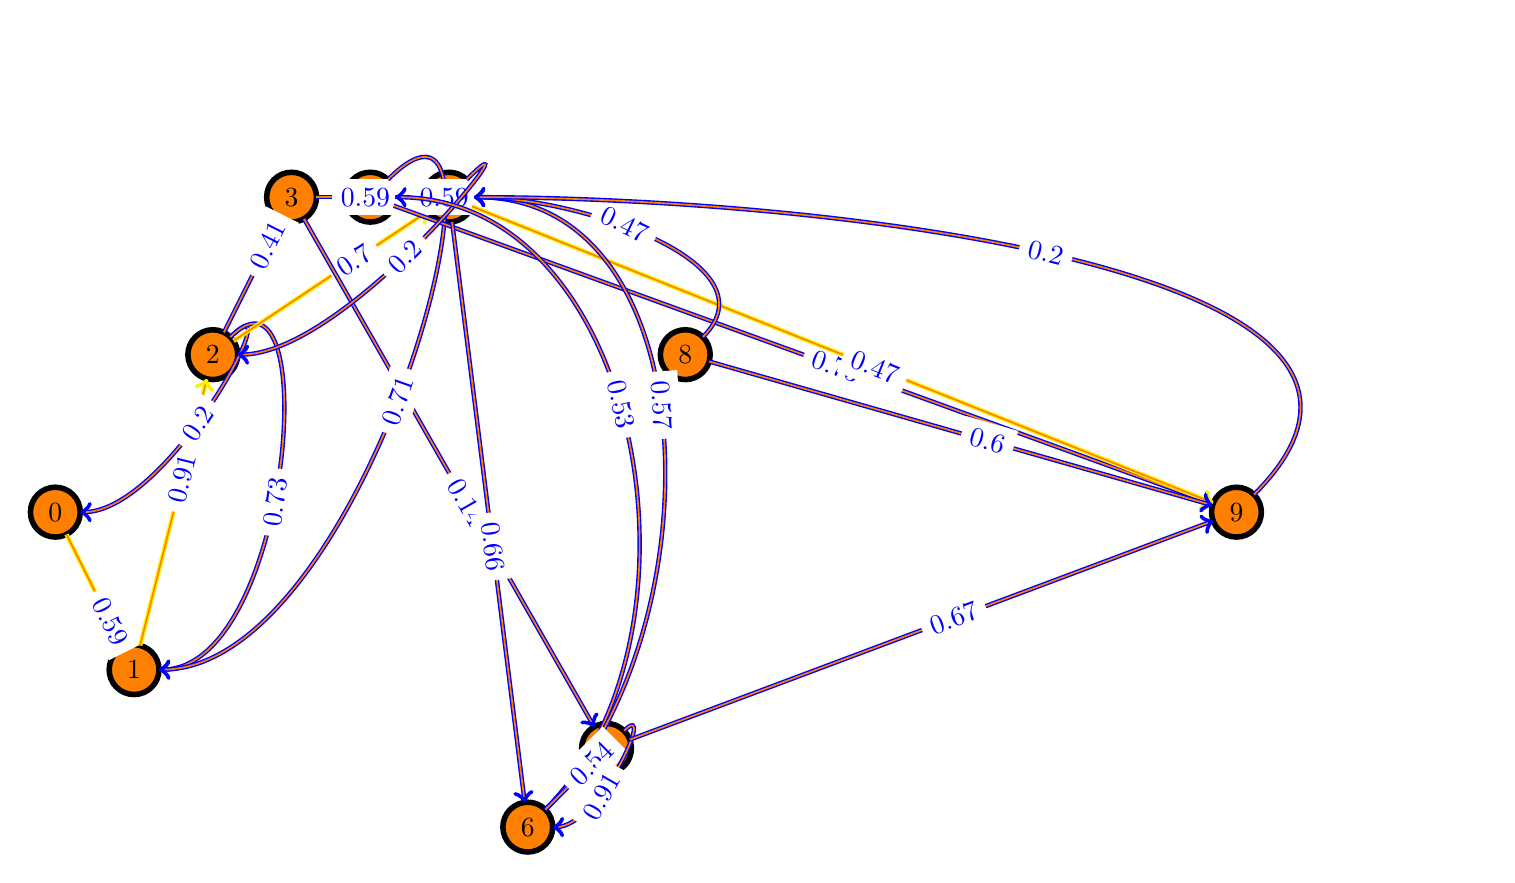
\begin{tikzpicture}
\SetVertexNormal[Shape      = circle,
FillColor  = orange,
LineWidth  = 2pt]
\SetUpEdge[lw         = 0.5pt,
color      = black,
labelcolor = white,
labeltext  = red,
labelstyle = {sloped,text=blue}]
\tikzstyle{TempStyle}=[double = orange]
\Vertex[x=-10, y=8]{0}
\Vertex[x=-9, y=6]{1}
\Vertex[x=-8, y=10]{2}
\Vertex[x=-7, y=12]{3}
\Vertex[x=-6, y=12]{4}
\Vertex[x=-5, y=12]{5}
\Vertex[x=-4, y=4]{6}
\Vertex[x=-3, y=5]{7}
\Vertex[x=-2, y=10]{8}
\Vertex[x=5, y=8]{9}
\tikzset{EdgeStyle/.style={->,TempStyle,relative=false,right=60,color=yellow}}
\Edge[label=$0.59$](0)(1)
\tikzset{EdgeStyle/.style={->,TempStyle,relative=false,right=60,color=yellow}}
\Edge[label=$0.91$](1)(2)
\tikzset{EdgeStyle/.style={->,TempStyle,relative=false,left=60,color=blue,in=0,draw}}
\Edge[label=$0.2$](2)(0)
\tikzset{EdgeStyle/.style={->,TempStyle,relative=false,left=60,color=blue,in=0,draw}}
\Edge[label=$0.73$](2)(1)
\tikzset{EdgeStyle/.style={->,TempStyle,relative=false,right=60,color=blue}}
\Edge[label=$0.41$](2)(3)
\tikzset{EdgeStyle/.style={->,TempStyle,relative=false,right=60,color=yellow}}
\Edge[label=$0.7$](2)(5)
\tikzset{EdgeStyle/.style={->,TempStyle,relative=false,right=60,color=blue}}
\Edge[label=$0.59$](3)(4)
\tikzset{EdgeStyle/.style={->,TempStyle,relative=false,right=60,color=blue}}
\Edge[label=$0.14$](3)(7)
\tikzset{EdgeStyle/.style={->,TempStyle,relative=false,left=60,color=blue,in=0,draw}}
\Edge[label=$0.71$](4)(1)
\tikzset{EdgeStyle/.style={->,TempStyle,relative=false,right=60,color=blue}}
\Edge[label=$0.59$](4)(5)
\tikzset{EdgeStyle/.style={->,TempStyle,relative=false,right=60,color=blue}}
\Edge[label=$0.73$](4)(9)
\tikzset{EdgeStyle/.style={->,TempStyle,relative=false,left=60,color=blue,in=0,draw}}
\Edge[label=$0.2$](5)(2)
\tikzset{EdgeStyle/.style={->,TempStyle,relative=false,right=60,color=blue}}
\Edge[label=$0.66$](5)(6)
\tikzset{EdgeStyle/.style={->,TempStyle,relative=false,right=60,color=yellow}}
\Edge[label=$0.47$](5)(9)
\tikzset{EdgeStyle/.style={->,TempStyle,relative=false,left=60,color=blue,in=0,draw}}
\Edge[label=$0.53$](6)(4)
\tikzset{EdgeStyle/.style={->,TempStyle,relative=false,left=60,color=blue,in=0,draw}}
\Edge[label=$0.57$](6)(5)
\tikzset{EdgeStyle/.style={->,TempStyle,relative=false,right=60,color=blue}}
\Edge[label=$0.54$](6)(7)
\tikzset{EdgeStyle/.style={->,TempStyle,relative=false,left=60,color=blue,in=0,draw}}
\Edge[label=$0.91$](7)(6)
\tikzset{EdgeStyle/.style={->,TempStyle,relative=false,right=60,color=blue}}
\Edge[label=$0.67$](7)(9)
\tikzset{EdgeStyle/.style={->,TempStyle,relative=false,left=60,color=blue,in=0,draw}}
\Edge[label=$0.47$](8)(5)
\tikzset{EdgeStyle/.style={->,TempStyle,relative=false,right=60,color=blue}}
\Edge[label=$0.6$](8)(9)
\tikzset{EdgeStyle/.style={->,TempStyle,relative=false,left=60,color=blue,in=0,draw}}
\Edge[label=$0.2$](9)(5)
\end{tikzpicture}\\
\begin{center}\begin{tabular}{l c}\\
\textcolor{orange}{\LARGE$\rightarrow$} & Chemin \\
 \textcolor{red}{\LARGE$\rightarrow$} & Créations arcs\\
 \textcolor{green}{\LARGE$\rightarrow$} & Modification flot\\
\end{tabular}
\end{center}
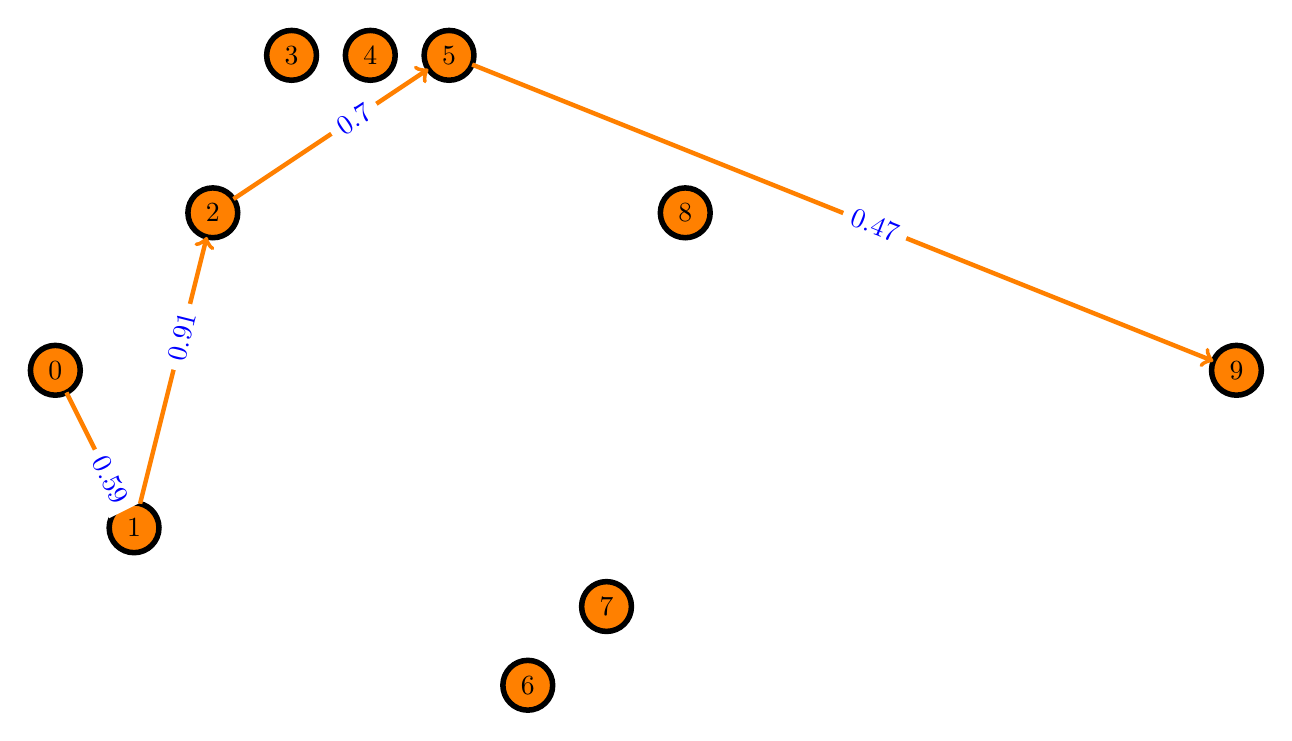
\begin{tikzpicture}
\SetVertexNormal[Shape      = circle,
FillColor  = orange,
LineWidth  = 2pt]
\SetUpEdge[lw         = 0.5pt,
color      = black,
labelcolor = white,
labeltext  = red,
labelstyle = {sloped,text=blue}]
\tikzstyle{TempStyle}=[double = orange]
\Vertex[x=-10, y=8]{0}
\Vertex[x=-9, y=6]{1}
\Vertex[x=-8, y=10]{2}
\Vertex[x=-7, y=12]{3}
\Vertex[x=-6, y=12]{4}
\Vertex[x=-5, y=12]{5}
\Vertex[x=-4, y=4]{6}
\Vertex[x=-3, y=5]{7}
\Vertex[x=-2, y=10]{8}
\Vertex[x=5, y=8]{9}
\tikzset{EdgeStyle/.style={->,TempStyle,relative=false,right=60,color=orange}}
\Edge[label=$0.59$](0)(1)
\tikzset{EdgeStyle/.style={->,TempStyle,relative=false,right=60,color=orange}}
\Edge[label=$0.91$](1)(2)
\tikzset{EdgeStyle/.style={->,TempStyle,relative=false,right=60,color=orange}}
\Edge[label=$0.7$](2)(5)
\tikzset{EdgeStyle/.style={->,TempStyle,relative=false,right=60,color=orange}}
\Edge[label=$0.47$](5)(9)
\end{tikzpicture}\\
\begin{center}\begin{tabular}{l c}\\
\textcolor{orange}{\LARGE$\rightarrow$} & Chemin \\
 \textcolor{red}{\LARGE$\rightarrow$} & Créations arcs\\
 \textcolor{green}{\LARGE$\rightarrow$} & Modification flot\\
\end{tabular}
\end{center}
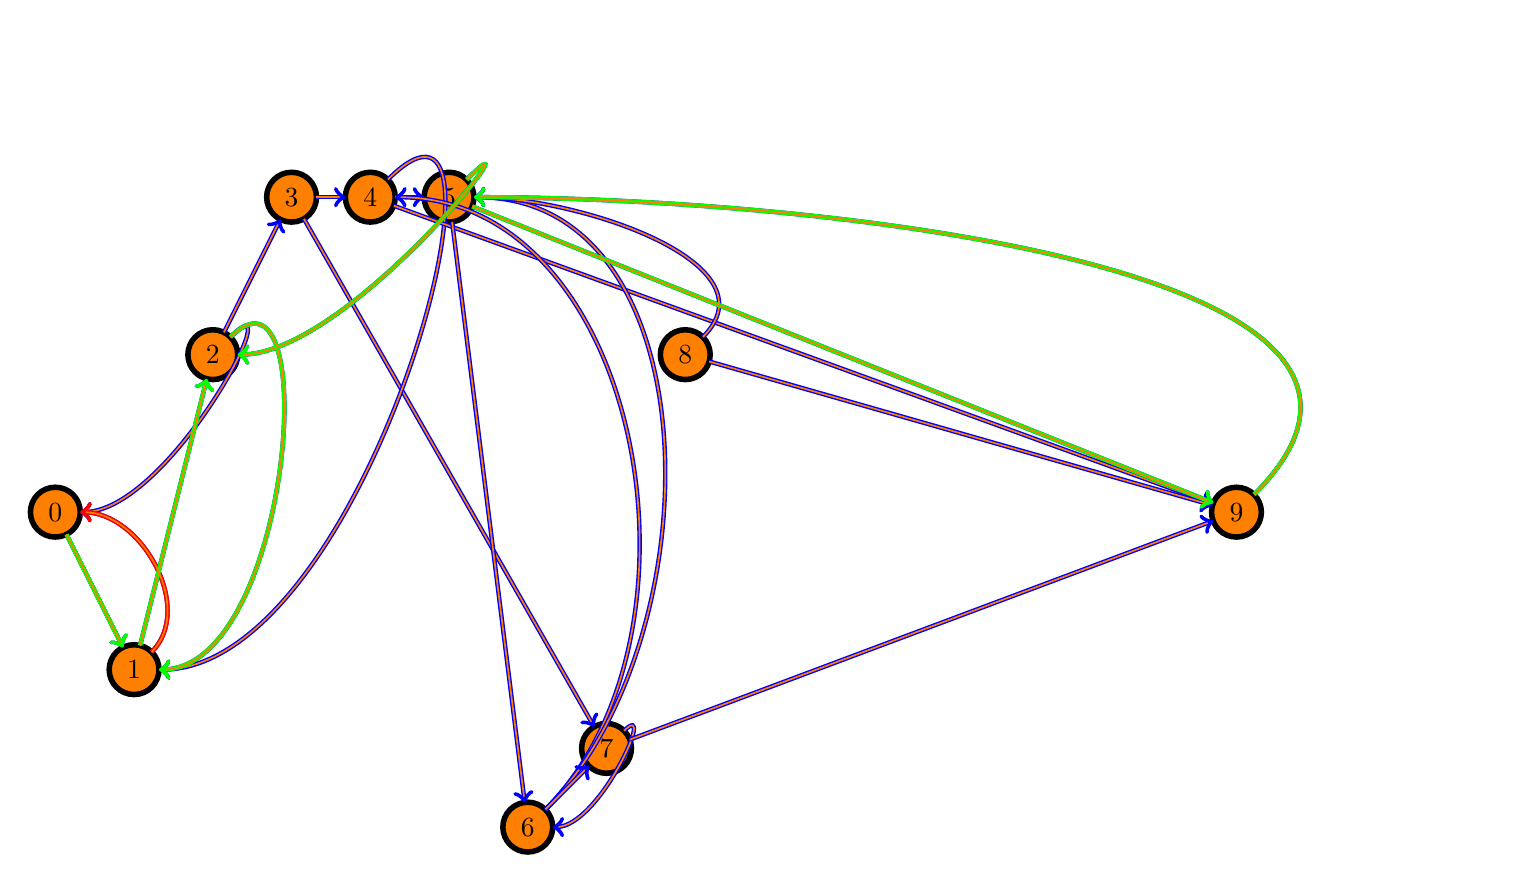
\begin{tikzpicture}
\SetVertexNormal[Shape      = circle,
FillColor  = orange,
LineWidth  = 2pt]
\SetUpEdge[lw         = 0.5pt,
color      = black,
labelcolor = white,
labeltext  = red,
labelstyle = {sloped,text=blue}]
\tikzstyle{TempStyle}=[double = orange]
\Vertex[x=-10, y=8]{0}
\Vertex[x=-9, y=6]{1}
\Vertex[x=-8, y=10]{2}
\Vertex[x=-7, y=12]{3}
\Vertex[x=-6, y=12]{4}
\Vertex[x=-5, y=12]{5}
\Vertex[x=-4, y=4]{6}
\Vertex[x=-3, y=5]{7}
\Vertex[x=-2, y=10]{8}
\Vertex[x=5, y=8]{9}
\tikzset{EdgeStyle/.style={->,TempStyle,relative=false,right=60,color=blue}}
\Edge(0)(1)
\tikzset{EdgeStyle/.style={->,TempStyle,relative=false,left=60,color=blue,in=0,draw}}
\Edge(1)(0)
\tikzset{EdgeStyle/.style={->,TempStyle,relative=false,right=60,color=blue}}
\Edge(1)(2)
\tikzset{EdgeStyle/.style={->,TempStyle,relative=false,left=60,color=blue,in=0,draw}}
\Edge(2)(0)
\tikzset{EdgeStyle/.style={->,TempStyle,relative=false,left=60,color=blue,in=0,draw}}
\Edge(2)(1)
\tikzset{EdgeStyle/.style={->,TempStyle,relative=false,right=60,color=blue}}
\Edge(2)(3)
\tikzset{EdgeStyle/.style={->,TempStyle,relative=false,right=60,color=blue}}
\Edge(3)(4)
\tikzset{EdgeStyle/.style={->,TempStyle,relative=false,right=60,color=blue}}
\Edge(3)(7)
\tikzset{EdgeStyle/.style={->,TempStyle,relative=false,left=60,color=blue,in=0,draw}}
\Edge(4)(1)
\tikzset{EdgeStyle/.style={->,TempStyle,relative=false,right=60,color=blue}}
\Edge(4)(5)
\tikzset{EdgeStyle/.style={->,TempStyle,relative=false,right=60,color=blue}}
\Edge(4)(9)
\tikzset{EdgeStyle/.style={->,TempStyle,relative=false,left=60,color=blue,in=0,draw}}
\Edge(5)(2)
\tikzset{EdgeStyle/.style={->,TempStyle,relative=false,right=60,color=blue}}
\Edge(5)(6)
\tikzset{EdgeStyle/.style={->,TempStyle,relative=false,right=60,color=blue}}
\Edge(5)(9)
\tikzset{EdgeStyle/.style={->,TempStyle,relative=false,left=60,color=blue,in=0,draw}}
\Edge(6)(4)
\tikzset{EdgeStyle/.style={->,TempStyle,relative=false,left=60,color=blue,in=0,draw}}
\Edge(6)(5)
\tikzset{EdgeStyle/.style={->,TempStyle,relative=false,right=60,color=blue}}
\Edge(6)(7)
\tikzset{EdgeStyle/.style={->,TempStyle,relative=false,left=60,color=blue,in=0,draw}}
\Edge(7)(6)
\tikzset{EdgeStyle/.style={->,TempStyle,relative=false,right=60,color=blue}}
\Edge(7)(9)
\tikzset{EdgeStyle/.style={->,TempStyle,relative=false,left=60,color=blue,in=0,draw}}
\Edge(8)(5)
\tikzset{EdgeStyle/.style={->,TempStyle,relative=false,right=60,color=blue}}
\Edge(8)(9)
\tikzset{EdgeStyle/.style={->,TempStyle,relative=false,left=60,color=blue,in=0,draw}}
\Edge(9)(5)
\tikzset{EdgeStyle/.style={->,TempStyle,relative=false,right=60,color=green}}
\Edge(0)(1)
\tikzset{EdgeStyle/.style={->,TempStyle,relative=false,right=60,in=0,color=red}}
\Edge(1)(0)
\tikzset{EdgeStyle/.style={->,TempStyle,relative=false,right=60,color=green}}
\Edge(1)(2)
\tikzset{EdgeStyle/.style={->,TempStyle,relative=false,right=60,in=0,color=green}}
\Edge(2)(1)
\tikzset{EdgeStyle/.style={->,TempStyle,relative=false,right=60,in=0,color=green}}
\Edge(5)(2)
\tikzset{EdgeStyle/.style={->,TempStyle,relative=false,right=60,color=green}}
\Edge(5)(9)
\tikzset{EdgeStyle/.style={->,TempStyle,relative=false,right=60,in=0,color=green}}
\Edge(9)(5)
\end{tikzpicture}\\
\begin{center}\begin{tabular}{l c}\\
\textcolor{orange}{\LARGE$\rightarrow$} & Chemin \\
 \textcolor{red}{\LARGE$\rightarrow$} & Créations arcs\\
 \textcolor{green}{\LARGE$\rightarrow$} & Modification flot\\
\end{tabular}
\end{center}
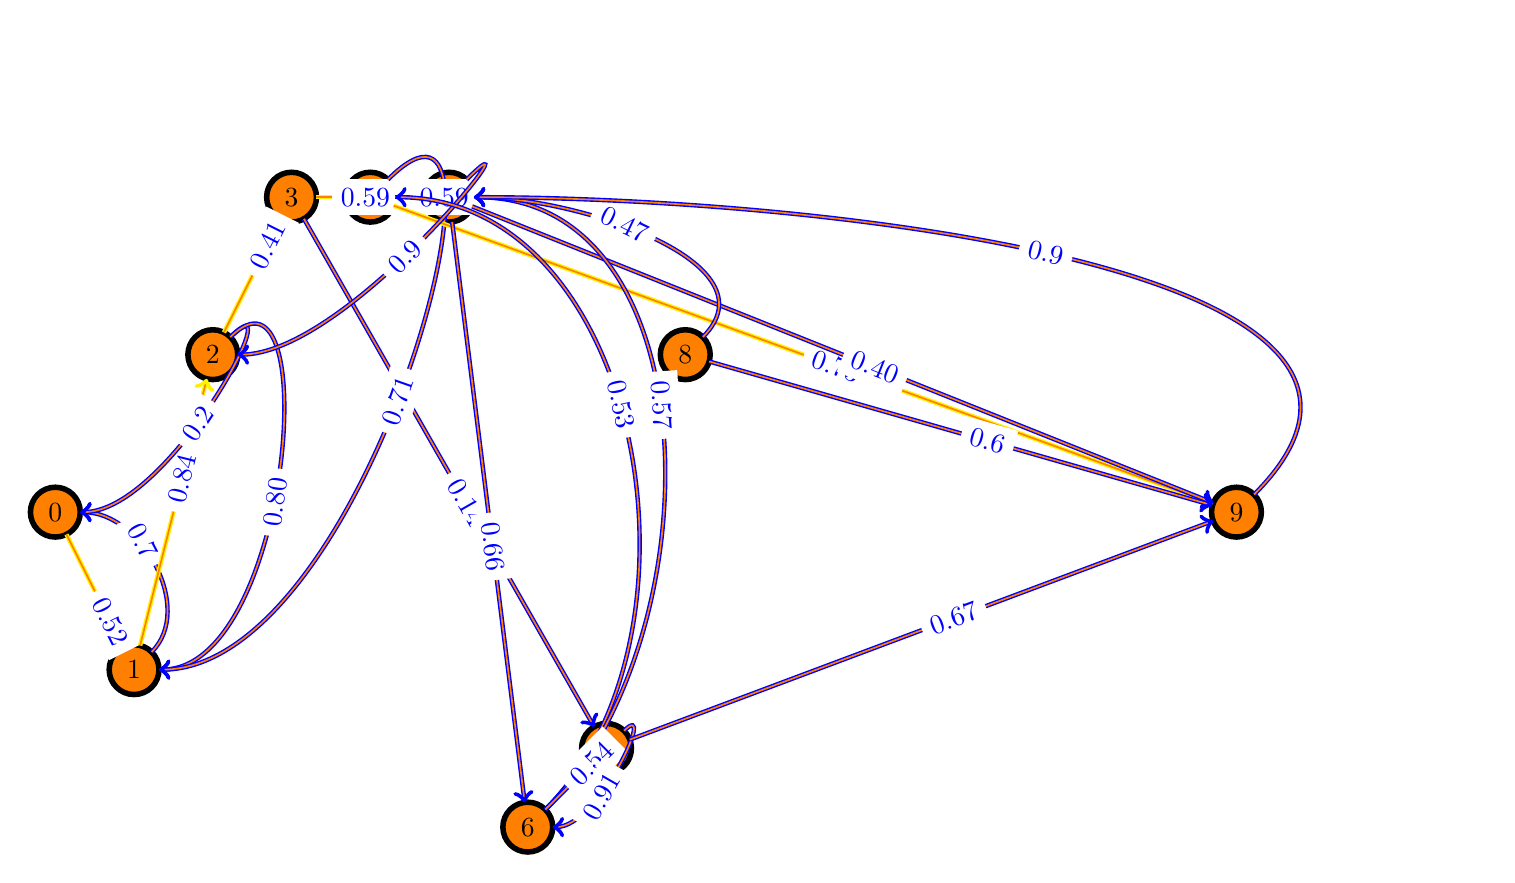
\begin{tikzpicture}
\SetVertexNormal[Shape      = circle,
FillColor  = orange,
LineWidth  = 2pt]
\SetUpEdge[lw         = 0.5pt,
color      = black,
labelcolor = white,
labeltext  = red,
labelstyle = {sloped,text=blue}]
\tikzstyle{TempStyle}=[double = orange]
\Vertex[x=-10, y=8]{0}
\Vertex[x=-9, y=6]{1}
\Vertex[x=-8, y=10]{2}
\Vertex[x=-7, y=12]{3}
\Vertex[x=-6, y=12]{4}
\Vertex[x=-5, y=12]{5}
\Vertex[x=-4, y=4]{6}
\Vertex[x=-3, y=5]{7}
\Vertex[x=-2, y=10]{8}
\Vertex[x=5, y=8]{9}
\tikzset{EdgeStyle/.style={->,TempStyle,relative=false,right=60,color=yellow}}
\Edge[label=$0.52$](0)(1)
\tikzset{EdgeStyle/.style={->,TempStyle,relative=false,left=60,color=blue,in=0,draw}}
\Edge[label=$0.7$](1)(0)
\tikzset{EdgeStyle/.style={->,TempStyle,relative=false,right=60,color=yellow}}
\Edge[label=$0.84$](1)(2)
\tikzset{EdgeStyle/.style={->,TempStyle,relative=false,left=60,color=blue,in=0,draw}}
\Edge[label=$0.2$](2)(0)
\tikzset{EdgeStyle/.style={->,TempStyle,relative=false,left=60,color=blue,in=0,draw}}
\Edge[label=$0.80$](2)(1)
\tikzset{EdgeStyle/.style={->,TempStyle,relative=false,right=60,color=yellow}}
\Edge[label=$0.41$](2)(3)
\tikzset{EdgeStyle/.style={->,TempStyle,relative=false,right=60,color=yellow}}
\Edge[label=$0.59$](3)(4)
\tikzset{EdgeStyle/.style={->,TempStyle,relative=false,right=60,color=blue}}
\Edge[label=$0.14$](3)(7)
\tikzset{EdgeStyle/.style={->,TempStyle,relative=false,left=60,color=blue,in=0,draw}}
\Edge[label=$0.71$](4)(1)
\tikzset{EdgeStyle/.style={->,TempStyle,relative=false,right=60,color=blue}}
\Edge[label=$0.59$](4)(5)
\tikzset{EdgeStyle/.style={->,TempStyle,relative=false,right=60,color=yellow}}
\Edge[label=$0.73$](4)(9)
\tikzset{EdgeStyle/.style={->,TempStyle,relative=false,left=60,color=blue,in=0,draw}}
\Edge[label=$0.9$](5)(2)
\tikzset{EdgeStyle/.style={->,TempStyle,relative=false,right=60,color=blue}}
\Edge[label=$0.66$](5)(6)
\tikzset{EdgeStyle/.style={->,TempStyle,relative=false,right=60,color=blue}}
\Edge[label=$0.40$](5)(9)
\tikzset{EdgeStyle/.style={->,TempStyle,relative=false,left=60,color=blue,in=0,draw}}
\Edge[label=$0.53$](6)(4)
\tikzset{EdgeStyle/.style={->,TempStyle,relative=false,left=60,color=blue,in=0,draw}}
\Edge[label=$0.57$](6)(5)
\tikzset{EdgeStyle/.style={->,TempStyle,relative=false,right=60,color=blue}}
\Edge[label=$0.54$](6)(7)
\tikzset{EdgeStyle/.style={->,TempStyle,relative=false,left=60,color=blue,in=0,draw}}
\Edge[label=$0.91$](7)(6)
\tikzset{EdgeStyle/.style={->,TempStyle,relative=false,right=60,color=blue}}
\Edge[label=$0.67$](7)(9)
\tikzset{EdgeStyle/.style={->,TempStyle,relative=false,left=60,color=blue,in=0,draw}}
\Edge[label=$0.47$](8)(5)
\tikzset{EdgeStyle/.style={->,TempStyle,relative=false,right=60,color=blue}}
\Edge[label=$0.6$](8)(9)
\tikzset{EdgeStyle/.style={->,TempStyle,relative=false,left=60,color=blue,in=0,draw}}
\Edge[label=$0.9$](9)(5)
\end{tikzpicture}\\
\begin{center}\begin{tabular}{l c}\\
\textcolor{orange}{\LARGE$\rightarrow$} & Chemin \\
 \textcolor{red}{\LARGE$\rightarrow$} & Créations arcs\\
 \textcolor{green}{\LARGE$\rightarrow$} & Modification flot\\
\end{tabular}
\end{center}
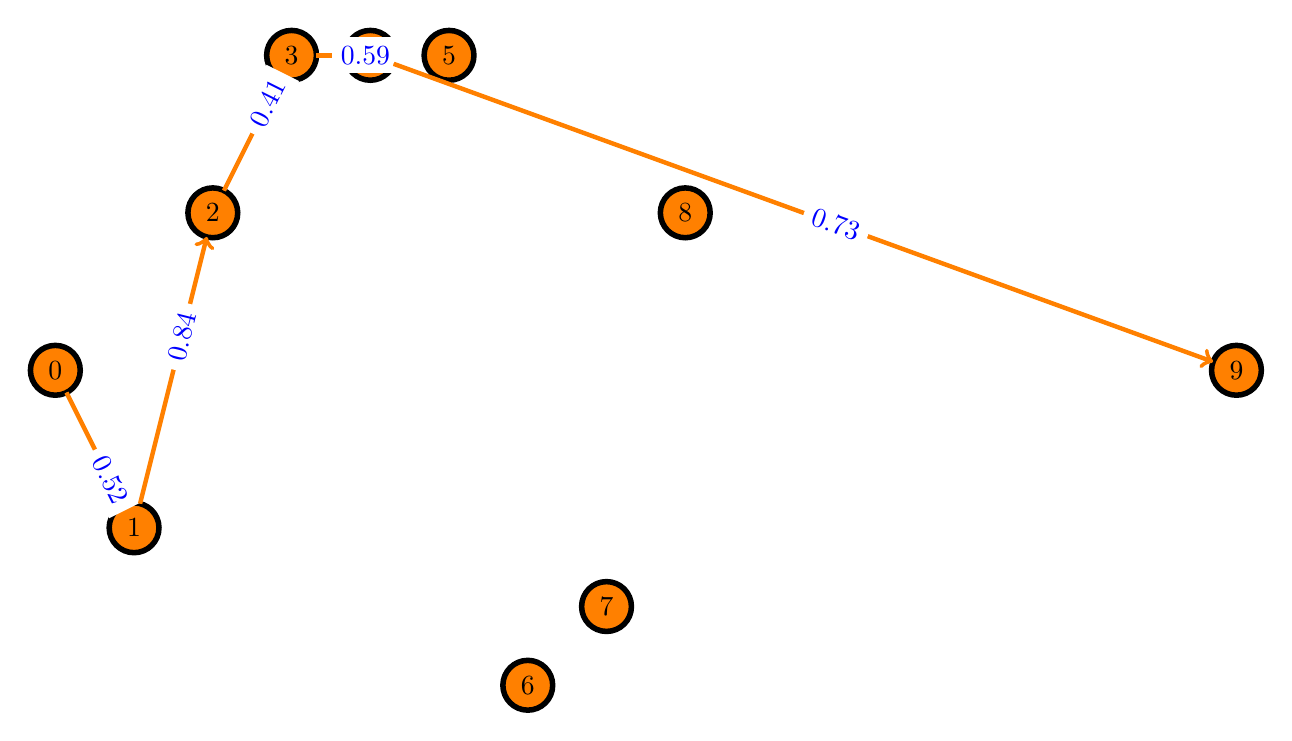
\begin{tikzpicture}
\SetVertexNormal[Shape      = circle,
FillColor  = orange,
LineWidth  = 2pt]
\SetUpEdge[lw         = 0.5pt,
color      = black,
labelcolor = white,
labeltext  = red,
labelstyle = {sloped,text=blue}]
\tikzstyle{TempStyle}=[double = orange]
\Vertex[x=-10, y=8]{0}
\Vertex[x=-9, y=6]{1}
\Vertex[x=-8, y=10]{2}
\Vertex[x=-7, y=12]{3}
\Vertex[x=-6, y=12]{4}
\Vertex[x=-5, y=12]{5}
\Vertex[x=-4, y=4]{6}
\Vertex[x=-3, y=5]{7}
\Vertex[x=-2, y=10]{8}
\Vertex[x=5, y=8]{9}
\tikzset{EdgeStyle/.style={->,TempStyle,relative=false,right=60,color=orange}}
\Edge[label=$0.52$](0)(1)
\tikzset{EdgeStyle/.style={->,TempStyle,relative=false,right=60,color=orange}}
\Edge[label=$0.84$](1)(2)
\tikzset{EdgeStyle/.style={->,TempStyle,relative=false,right=60,color=orange}}
\Edge[label=$0.41$](2)(3)
\tikzset{EdgeStyle/.style={->,TempStyle,relative=false,right=60,color=orange}}
\Edge[label=$0.59$](3)(4)
\tikzset{EdgeStyle/.style={->,TempStyle,relative=false,right=60,color=orange}}
\Edge[label=$0.73$](4)(9)
\end{tikzpicture}\\
\begin{center}\begin{tabular}{l c}\\
\textcolor{orange}{\LARGE$\rightarrow$} & Chemin \\
 \textcolor{red}{\LARGE$\rightarrow$} & Créations arcs\\
 \textcolor{green}{\LARGE$\rightarrow$} & Modification flot\\
\end{tabular}
\end{center}
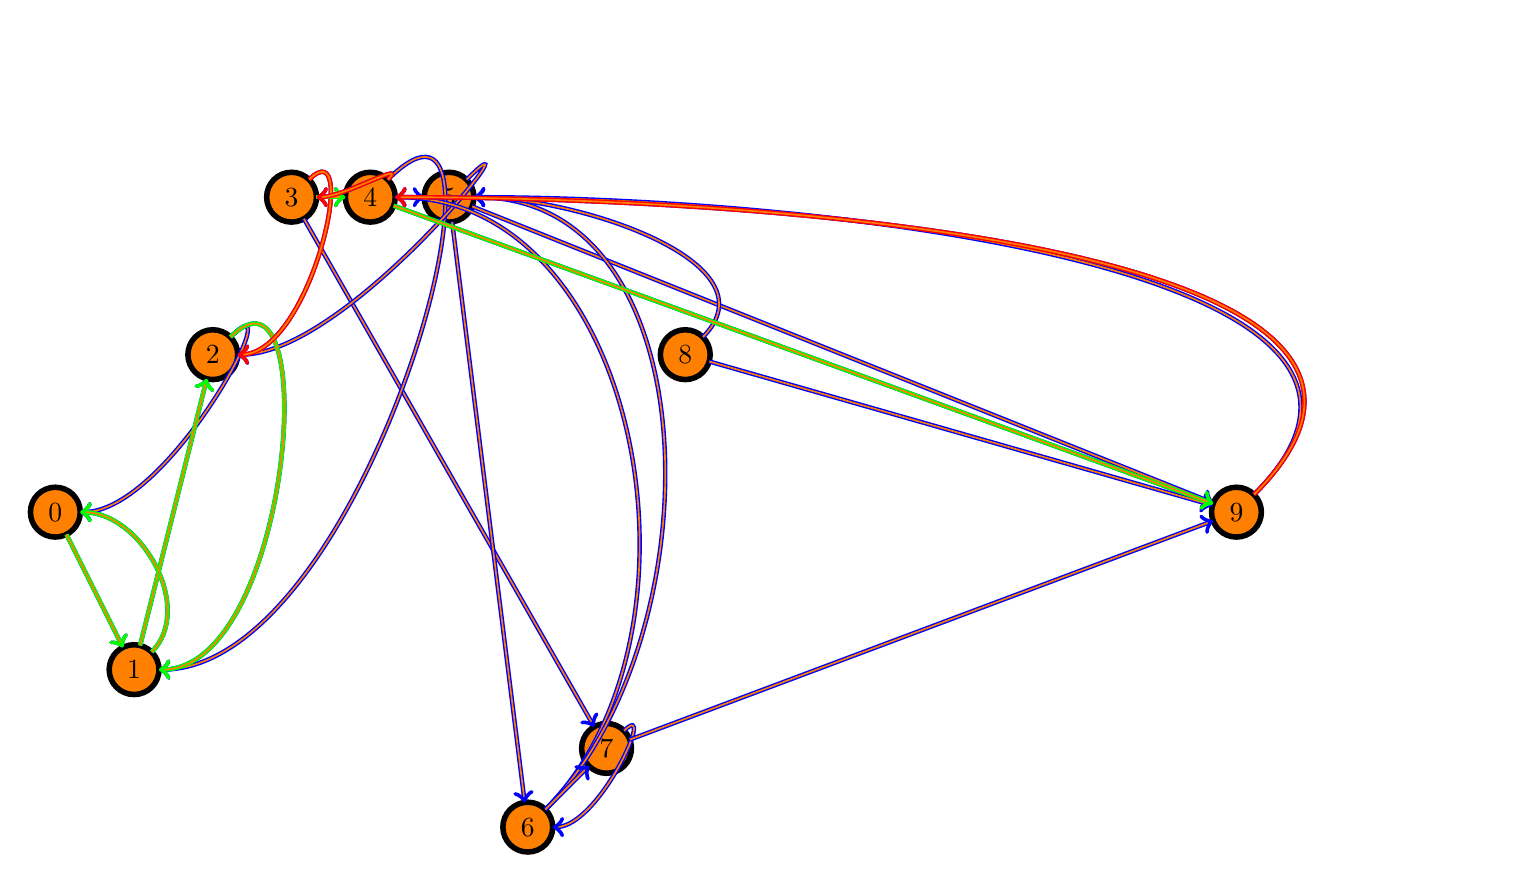
\begin{tikzpicture}
\SetVertexNormal[Shape      = circle,
FillColor  = orange,
LineWidth  = 2pt]
\SetUpEdge[lw         = 0.5pt,
color      = black,
labelcolor = white,
labeltext  = red,
labelstyle = {sloped,text=blue}]
\tikzstyle{TempStyle}=[double = orange]
\Vertex[x=-10, y=8]{0}
\Vertex[x=-9, y=6]{1}
\Vertex[x=-8, y=10]{2}
\Vertex[x=-7, y=12]{3}
\Vertex[x=-6, y=12]{4}
\Vertex[x=-5, y=12]{5}
\Vertex[x=-4, y=4]{6}
\Vertex[x=-3, y=5]{7}
\Vertex[x=-2, y=10]{8}
\Vertex[x=5, y=8]{9}
\tikzset{EdgeStyle/.style={->,TempStyle,relative=false,right=60,color=blue}}
\Edge(0)(1)
\tikzset{EdgeStyle/.style={->,TempStyle,relative=false,left=60,color=blue,in=0,draw}}
\Edge(1)(0)
\tikzset{EdgeStyle/.style={->,TempStyle,relative=false,right=60,color=blue}}
\Edge(1)(2)
\tikzset{EdgeStyle/.style={->,TempStyle,relative=false,left=60,color=blue,in=0,draw}}
\Edge(2)(0)
\tikzset{EdgeStyle/.style={->,TempStyle,relative=false,left=60,color=blue,in=0,draw}}
\Edge(2)(1)
\tikzset{EdgeStyle/.style={->,TempStyle,relative=false,left=60,color=blue,in=0,draw}}
\Edge(3)(2)
\tikzset{EdgeStyle/.style={->,TempStyle,relative=false,right=60,color=blue}}
\Edge(3)(4)
\tikzset{EdgeStyle/.style={->,TempStyle,relative=false,right=60,color=blue}}
\Edge(3)(7)
\tikzset{EdgeStyle/.style={->,TempStyle,relative=false,left=60,color=blue,in=0,draw}}
\Edge(4)(1)
\tikzset{EdgeStyle/.style={->,TempStyle,relative=false,left=60,color=blue,in=0,draw}}
\Edge(4)(3)
\tikzset{EdgeStyle/.style={->,TempStyle,relative=false,right=60,color=blue}}
\Edge(4)(5)
\tikzset{EdgeStyle/.style={->,TempStyle,relative=false,right=60,color=blue}}
\Edge(4)(9)
\tikzset{EdgeStyle/.style={->,TempStyle,relative=false,left=60,color=blue,in=0,draw}}
\Edge(5)(2)
\tikzset{EdgeStyle/.style={->,TempStyle,relative=false,right=60,color=blue}}
\Edge(5)(6)
\tikzset{EdgeStyle/.style={->,TempStyle,relative=false,right=60,color=blue}}
\Edge(5)(9)
\tikzset{EdgeStyle/.style={->,TempStyle,relative=false,left=60,color=blue,in=0,draw}}
\Edge(6)(4)
\tikzset{EdgeStyle/.style={->,TempStyle,relative=false,left=60,color=blue,in=0,draw}}
\Edge(6)(5)
\tikzset{EdgeStyle/.style={->,TempStyle,relative=false,right=60,color=blue}}
\Edge(6)(7)
\tikzset{EdgeStyle/.style={->,TempStyle,relative=false,left=60,color=blue,in=0,draw}}
\Edge(7)(6)
\tikzset{EdgeStyle/.style={->,TempStyle,relative=false,right=60,color=blue}}
\Edge(7)(9)
\tikzset{EdgeStyle/.style={->,TempStyle,relative=false,left=60,color=blue,in=0,draw}}
\Edge(8)(5)
\tikzset{EdgeStyle/.style={->,TempStyle,relative=false,right=60,color=blue}}
\Edge(8)(9)
\tikzset{EdgeStyle/.style={->,TempStyle,relative=false,left=60,color=blue,in=0,draw}}
\Edge(9)(4)
\tikzset{EdgeStyle/.style={->,TempStyle,relative=false,left=60,color=blue,in=0,draw}}
\Edge(9)(5)
\tikzset{EdgeStyle/.style={->,TempStyle,relative=false,right=60,color=green}}
\Edge(0)(1)
\tikzset{EdgeStyle/.style={->,TempStyle,relative=false,right=60,in=0,color=green}}
\Edge(1)(0)
\tikzset{EdgeStyle/.style={->,TempStyle,relative=false,right=60,color=green}}
\Edge(1)(2)
\tikzset{EdgeStyle/.style={->,TempStyle,relative=false,right=60,in=0,color=green}}
\Edge(2)(1)
\tikzset{EdgeStyle/.style={->,TempStyle,relative=false,right=60,in=0,color=red}}
\Edge(3)(2)
\tikzset{EdgeStyle/.style={->,TempStyle,relative=false,right=60,color=green}}
\Edge(3)(4)
\tikzset{EdgeStyle/.style={->,TempStyle,relative=false,right=60,in=0,color=red}}
\Edge(4)(3)
\tikzset{EdgeStyle/.style={->,TempStyle,relative=false,right=60,color=green}}
\Edge(4)(9)
\tikzset{EdgeStyle/.style={->,TempStyle,relative=false,right=60,in=0,color=red}}
\Edge(9)(4)
\end{tikzpicture}\\
\begin{center}\begin{tabular}{l c}\\
\textcolor{orange}{\LARGE$\rightarrow$} & Chemin \\
 \textcolor{red}{\LARGE$\rightarrow$} & Créations arcs\\
 \textcolor{green}{\LARGE$\rightarrow$} & Modification flot\\
\end{tabular}
\end{center}
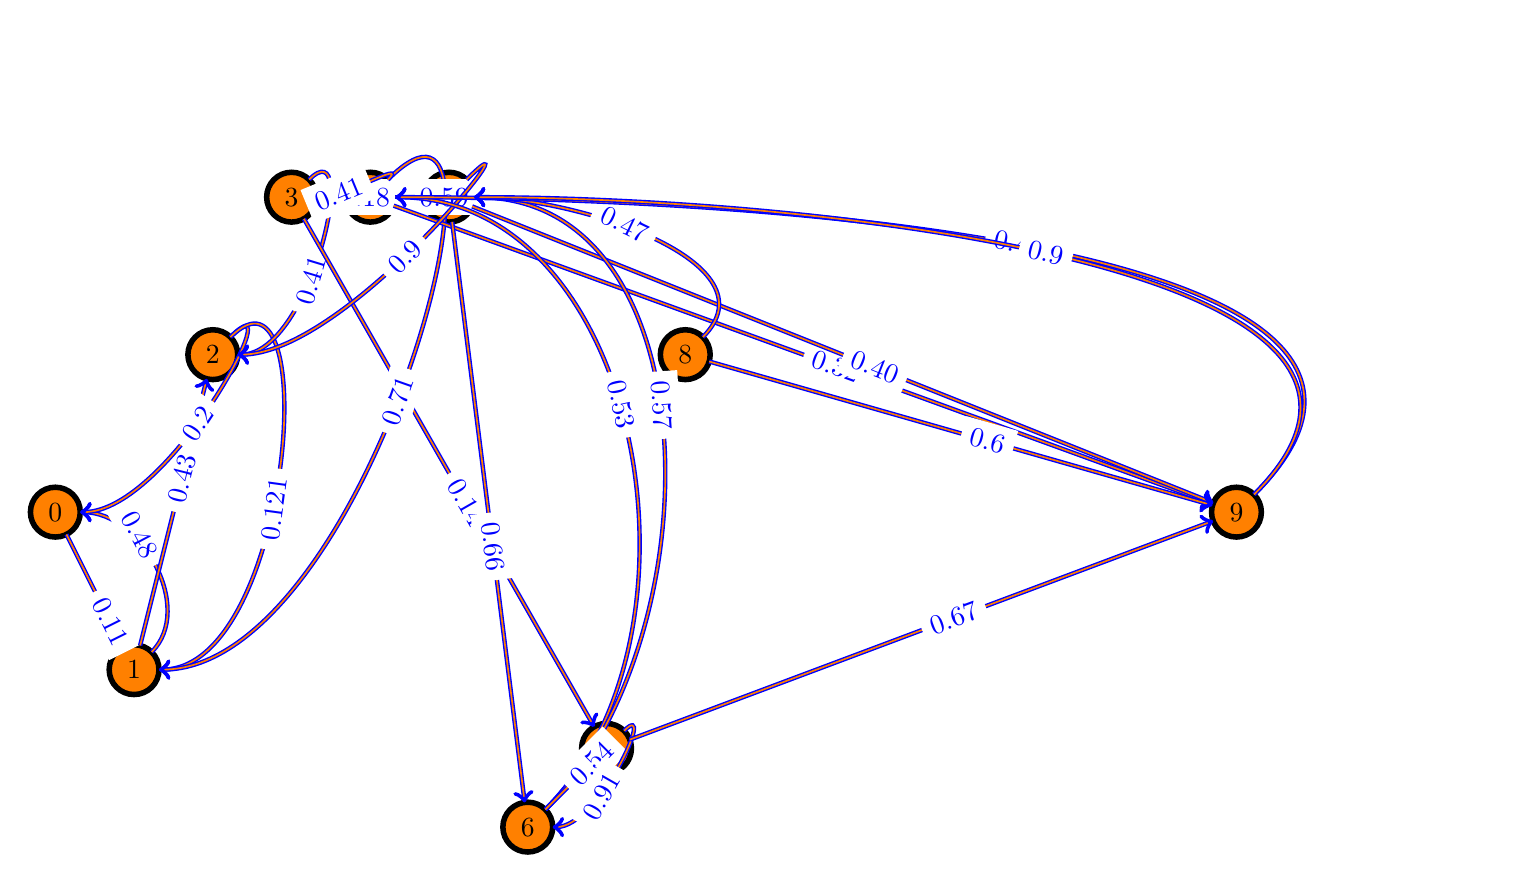
\begin{tikzpicture}
\SetVertexNormal[Shape      = circle,
FillColor  = orange,
LineWidth  = 2pt]
\SetUpEdge[lw         = 0.5pt,
color      = black,
labelcolor = white,
labeltext  = red,
labelstyle = {sloped,text=blue}]
\tikzstyle{TempStyle}=[double = orange]
\Vertex[x=-10, y=8]{0}
\Vertex[x=-9, y=6]{1}
\Vertex[x=-8, y=10]{2}
\Vertex[x=-7, y=12]{3}
\Vertex[x=-6, y=12]{4}
\Vertex[x=-5, y=12]{5}
\Vertex[x=-4, y=4]{6}
\Vertex[x=-3, y=5]{7}
\Vertex[x=-2, y=10]{8}
\Vertex[x=5, y=8]{9}
\tikzset{EdgeStyle/.style={->,TempStyle,relative=false,right=60,color=blue}}
\Edge[label=$0.11$](0)(1)
\tikzset{EdgeStyle/.style={->,TempStyle,relative=false,left=60,color=blue,in=0,draw}}
\Edge[label=$0.48$](1)(0)
\tikzset{EdgeStyle/.style={->,TempStyle,relative=false,right=60,color=blue}}
\Edge[label=$0.43$](1)(2)
\tikzset{EdgeStyle/.style={->,TempStyle,relative=false,left=60,color=blue,in=0,draw}}
\Edge[label=$0.2$](2)(0)
\tikzset{EdgeStyle/.style={->,TempStyle,relative=false,left=60,color=blue,in=0,draw}}
\Edge[label=$0.121$](2)(1)
\tikzset{EdgeStyle/.style={->,TempStyle,relative=false,left=60,color=blue,in=0,draw}}
\Edge[label=$0.41$](3)(2)
\tikzset{EdgeStyle/.style={->,TempStyle,relative=false,right=60,color=blue}}
\Edge[label=$0.18$](3)(4)
\tikzset{EdgeStyle/.style={->,TempStyle,relative=false,right=60,color=blue}}
\Edge[label=$0.14$](3)(7)
\tikzset{EdgeStyle/.style={->,TempStyle,relative=false,left=60,color=blue,in=0,draw}}
\Edge[label=$0.71$](4)(1)
\tikzset{EdgeStyle/.style={->,TempStyle,relative=false,left=60,color=blue,in=0,draw}}
\Edge[label=$0.41$](4)(3)
\tikzset{EdgeStyle/.style={->,TempStyle,relative=false,right=60,color=blue}}
\Edge[label=$0.59$](4)(5)
\tikzset{EdgeStyle/.style={->,TempStyle,relative=false,right=60,color=blue}}
\Edge[label=$0.32$](4)(9)
\tikzset{EdgeStyle/.style={->,TempStyle,relative=false,left=60,color=blue,in=0,draw}}
\Edge[label=$0.9$](5)(2)
\tikzset{EdgeStyle/.style={->,TempStyle,relative=false,right=60,color=blue}}
\Edge[label=$0.66$](5)(6)
\tikzset{EdgeStyle/.style={->,TempStyle,relative=false,right=60,color=blue}}
\Edge[label=$0.40$](5)(9)
\tikzset{EdgeStyle/.style={->,TempStyle,relative=false,left=60,color=blue,in=0,draw}}
\Edge[label=$0.53$](6)(4)
\tikzset{EdgeStyle/.style={->,TempStyle,relative=false,left=60,color=blue,in=0,draw}}
\Edge[label=$0.57$](6)(5)
\tikzset{EdgeStyle/.style={->,TempStyle,relative=false,right=60,color=blue}}
\Edge[label=$0.54$](6)(7)
\tikzset{EdgeStyle/.style={->,TempStyle,relative=false,left=60,color=blue,in=0,draw}}
\Edge[label=$0.91$](7)(6)
\tikzset{EdgeStyle/.style={->,TempStyle,relative=false,right=60,color=blue}}
\Edge[label=$0.67$](7)(9)
\tikzset{EdgeStyle/.style={->,TempStyle,relative=false,left=60,color=blue,in=0,draw}}
\Edge[label=$0.47$](8)(5)
\tikzset{EdgeStyle/.style={->,TempStyle,relative=false,right=60,color=blue}}
\Edge[label=$0.6$](8)(9)
\tikzset{EdgeStyle/.style={->,TempStyle,relative=false,left=60,color=blue,in=0,draw}}
\Edge[label=$0.41$](9)(4)
\tikzset{EdgeStyle/.style={->,TempStyle,relative=false,left=60,color=blue,in=0,draw}}
\Edge[label=$0.9$](9)(5)
\end{tikzpicture}\\
\begin{center}\begin{tabular}{l c}\\
\textcolor{orange}{\LARGE$\rightarrow$} & Chemin \\
 \textcolor{red}{\LARGE$\rightarrow$} & Créations arcs\\
 \textcolor{green}{\LARGE$\rightarrow$} & Modification flot\\
\end{tabular}
\end{center}
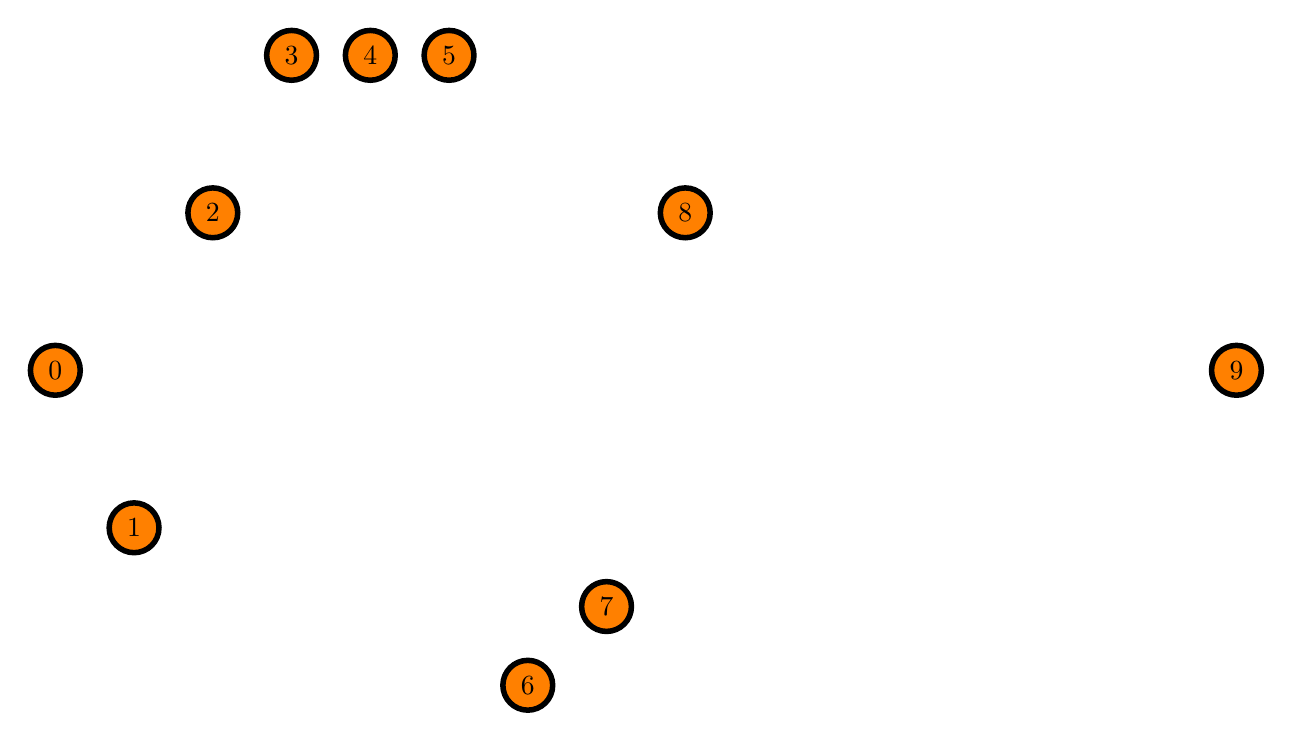
\begin{tikzpicture}
\SetVertexNormal[Shape      = circle,
FillColor  = orange,
LineWidth  = 2pt]
\SetUpEdge[lw         = 0.5pt,
color      = black,
labelcolor = white,
labeltext  = red,
labelstyle = {sloped,text=blue}]
\tikzstyle{TempStyle}=[double = orange]
\Vertex[x=-10, y=8]{0}
\Vertex[x=-9, y=6]{1}
\Vertex[x=-8, y=10]{2}
\Vertex[x=-7, y=12]{3}
\Vertex[x=-6, y=12]{4}
\Vertex[x=-5, y=12]{5}
\Vertex[x=-4, y=4]{6}
\Vertex[x=-3, y=5]{7}
\Vertex[x=-2, y=10]{8}
\Vertex[x=5, y=8]{9}
\end{tikzpicture}\\
\begin{center}\begin{tabular}{l c}\\
\textcolor{orange}{\LARGE$\rightarrow$} & Chemin \\
 \textcolor{red}{\LARGE$\rightarrow$} & Créations arcs\\
 \textcolor{green}{\LARGE$\rightarrow$} & Modification flot\\
\end{tabular}
\end{center}
\end{document}
